% Chapter Template

\chapter{Evidencias} % Main chapter title

\label{Chapter7} % Change X to a consecutive number; for referencing this chapter elsewhere, use \ref{ChapterX}

%----------------------------------------------------------------------------------------
%	SECTION 1
%----------------------------------------------------------------------------------------

\section{Pruebas de ejecución en universo Java}
Para hacer una prueba sencilla de ejecución en el universo Java, primero debemos crear un programa en java, compilarlo y luego enviarlo a la cola de trabajos de HTCondor. 

Para esta prueba usaremos un programa sencillo que hace un calculo y da una respuesta por terminal y luego veremos como se ejecuta este mismo trabajo en HTCondor.

\subsection{Creación y ejecución de la prueba}

primero creamos un archivo con nombre simple.java y lo editamos, y en el colocamos el contenido:
\begin{lstlisting}[frame=single,
  basicstyle=\footnotesize\ttfamily,
  language=Java, 
  numbers=left, 
  numberstyle=\tiny\color{black},
  captionpos=b]

\end{lstlisting}

\begin{figure}[h]
\centering
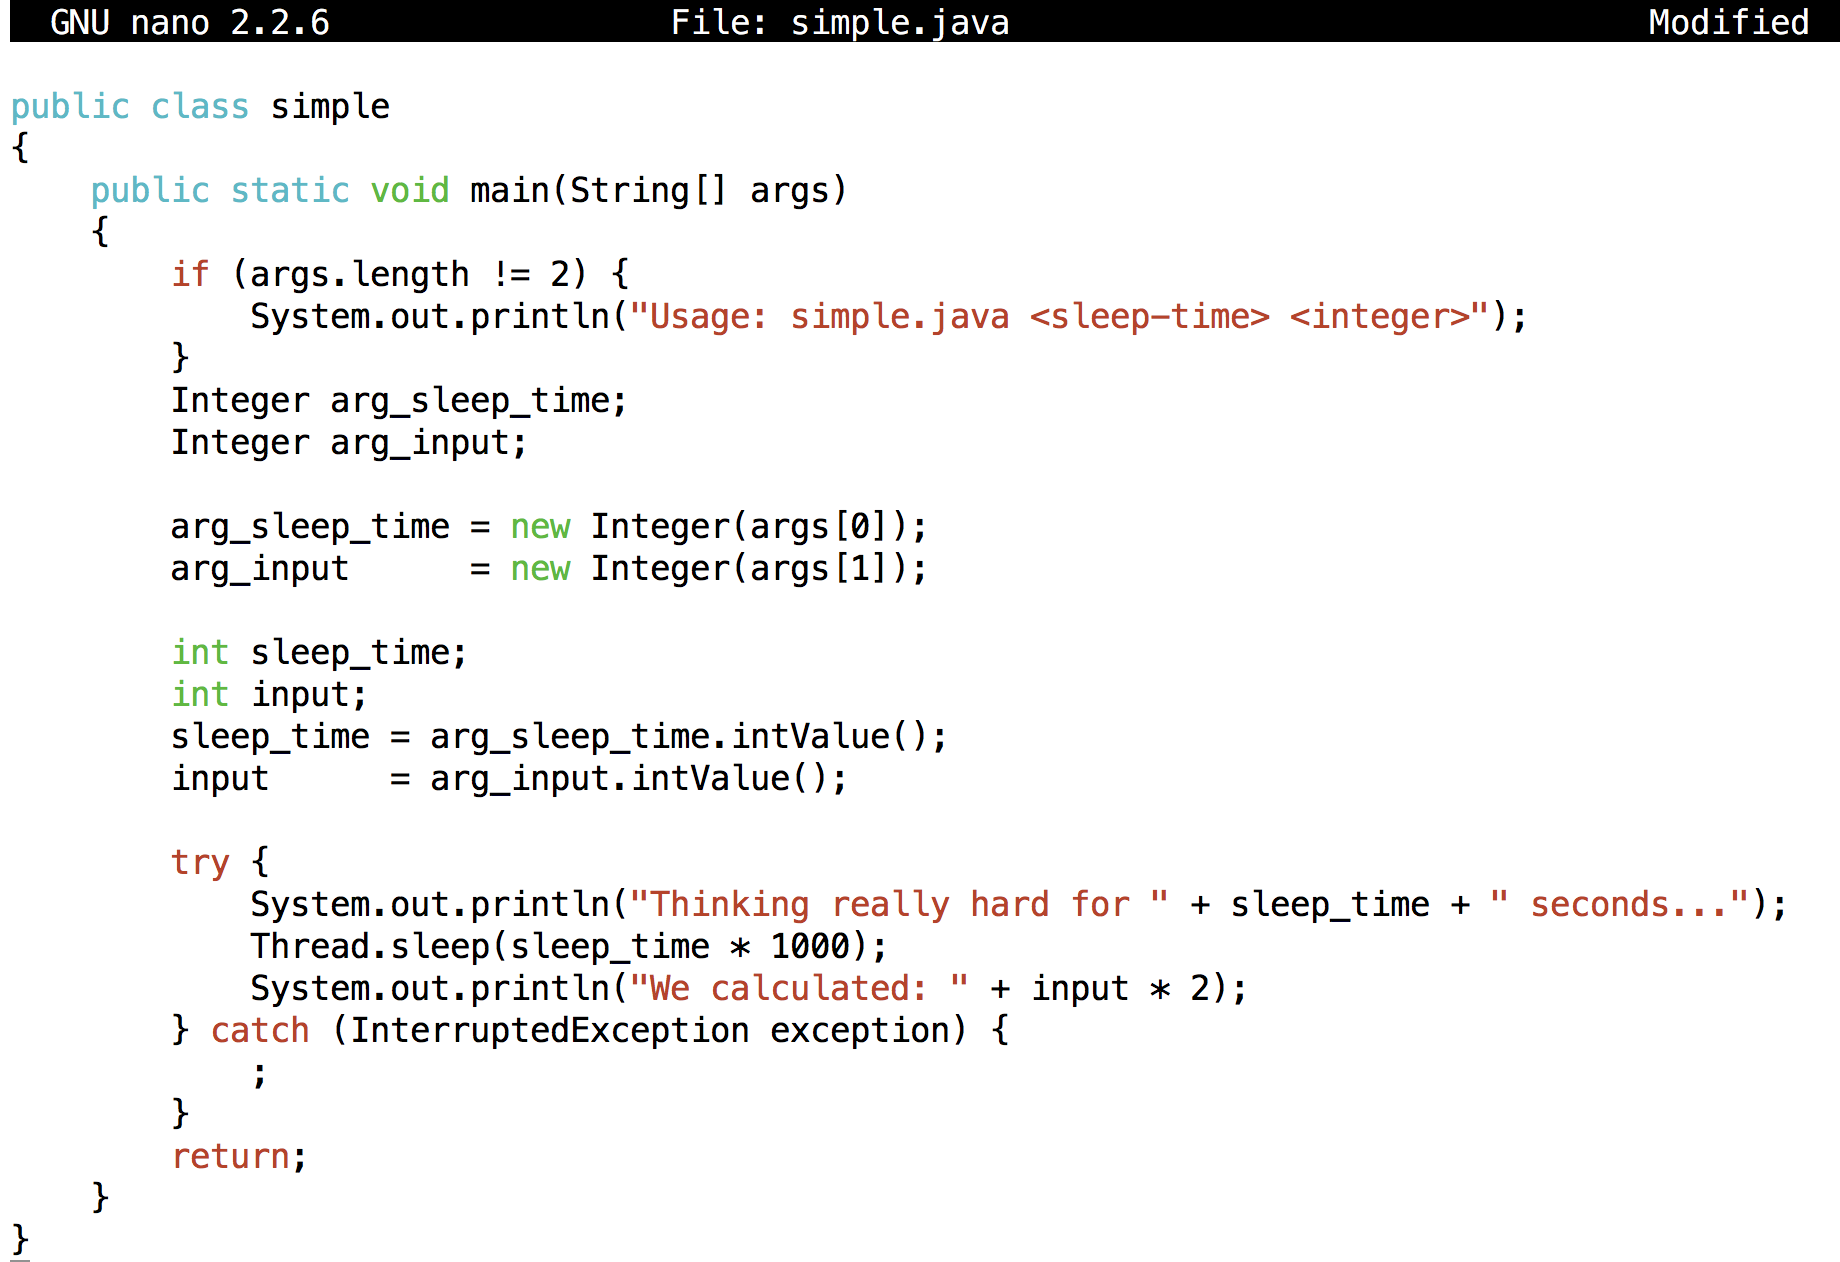
\includegraphics[width=0.9\textwidth]{images/simplejava.png}
\decoRule
\caption{Código prueba Java}
\label{fig:java test}
\end{figure}
\FloatBarrier


Luego compilamos el programa:

\textbf{javac simple.java}

Y lo ejecutamos:

\textbf{java simple 4 10}

nos arroja el resultado por terminal:

\begin{figure}[h]
\centering
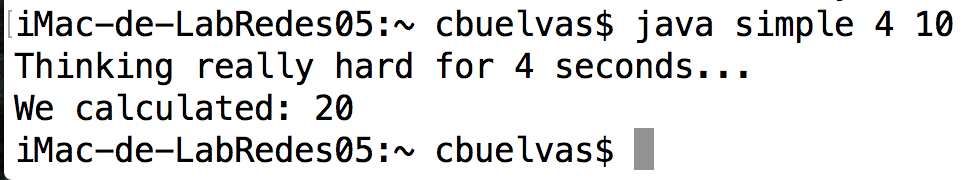
\includegraphics[width=0.8\textwidth]{images/resulttest.png}
\decoRule
\caption{Resultado ejecución local}
\label{fig:java test}
\end{figure}
\FloatBarrier

\subsection{Configuración de archivo ClassAd}

\subsubsection*{ClassAd}

HTCondor funciona mediante un mecanismo llamado \textbf{ClassAd},  este es un mecanismo flexible para la representación de las características y limitaciones de las máquinas y los trabajos (tareas) en HTCondor.
Dentro del sistema, los \textbf{ClassAd} pueden representar trabajos, recursos, nodos, máquinas remitentes y otros procesos de HTCondor.

Un ClassAd es un conjunto de expresiones de nombre exclusivo. Cada expresión nombrada se llama un atributo.

Enviamos a la maquina de envíos la prueba de java, y allí creamos el archivo de tarea que llamaremos \textbf{\textit{simple.job}}.

\textbf{Nota:} La extensión del archivo de tarea (submit file) puede ser cualquiera, luego que la configuración este realizada adecuadamente, utilizamos \textbf{.job} para mantener una idea clara de cual es su función.

El archivo de tarea quedara de la siguiente  manera.

\begin{lstlisting}[frame=single,
  basicstyle=\footnotesize\ttfamily,
  language=C, 
  numbers=left, 
  numberstyle=\tiny\color{black},
  captionpos=b]
Universe   = java
Executable = simple.class
Arguments  = simple 4 10
Log        = simple.log
Output     = simple.out.$(PROCESS)
Error      = simple.error
Rank       = (machine == "VMWorker24657")

should_transfer_files = YES
when_to_transfer_output = ON_EXIT

Queue 
\end{lstlisting}
  
Este archivo contiene toda la información necesaria para que HTCondor sepa donde ejecutar este trabajo. 

Los parámetros mostrados describen la configuración necesaria para la tarea.

\textbf{Universe}: Define el entorno de ejecución.

\textbf{Executable}: El archivo compilado que realizará la tarea 

\textbf{Arguments}: Los parámetros que recibe el archivo ejecutable.

\textbf{Log} : Crea un archivo con la información de la ejecución.

\textbf{Output}: Crea un archivo que contiene la salida de la ejecución.

\textbf{Error}: Crea un archivo de error con información en caso de fallas.

\textbf{Rank}: En esta prueba definimos que máquina del nodo queremos que ejecute la tarea.

\textbf{should\_transfer\_files} : define si se deben o no enviar archivos en el trabajo.

\textbf{when\_to\_transfer\_output}: especifica cuando transferir los resultados de la ejecución.

Para enviar el trabajo al cluster se usa el comando: \textit{\textbf{condor\_submit nombrearchivo.job}}

\begin{figure}[h]
\centering
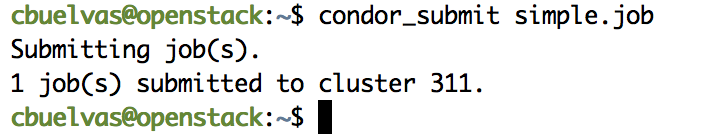
\includegraphics[width=0.8\textwidth]{images/submit.png}
\decoRule
\caption{Envío de trabajo al cluster}
\label{fig:condor submit}
\end{figure}
\FloatBarrier

Para verificar que el trabajo este en la cola se usa el comando : \textit{\textbf{condor\_q}}

\begin{figure}[h]
\centering
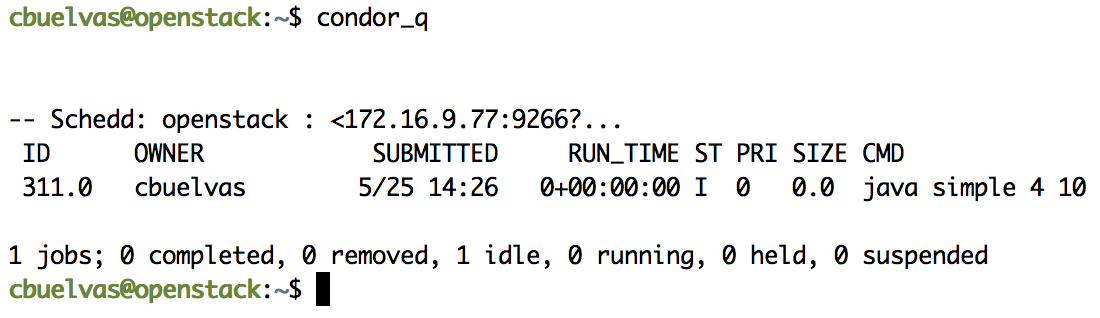
\includegraphics[width=1\textwidth]{images/condorq.png}
\decoRule
\caption{Cola de trabajo en el cluster}
\label{fig:condorq}
\end{figure}
\FloatBarrier

Verificación en el archivo simple.log del resultado de la ejecución.

\begin{figure}[h]
\centering
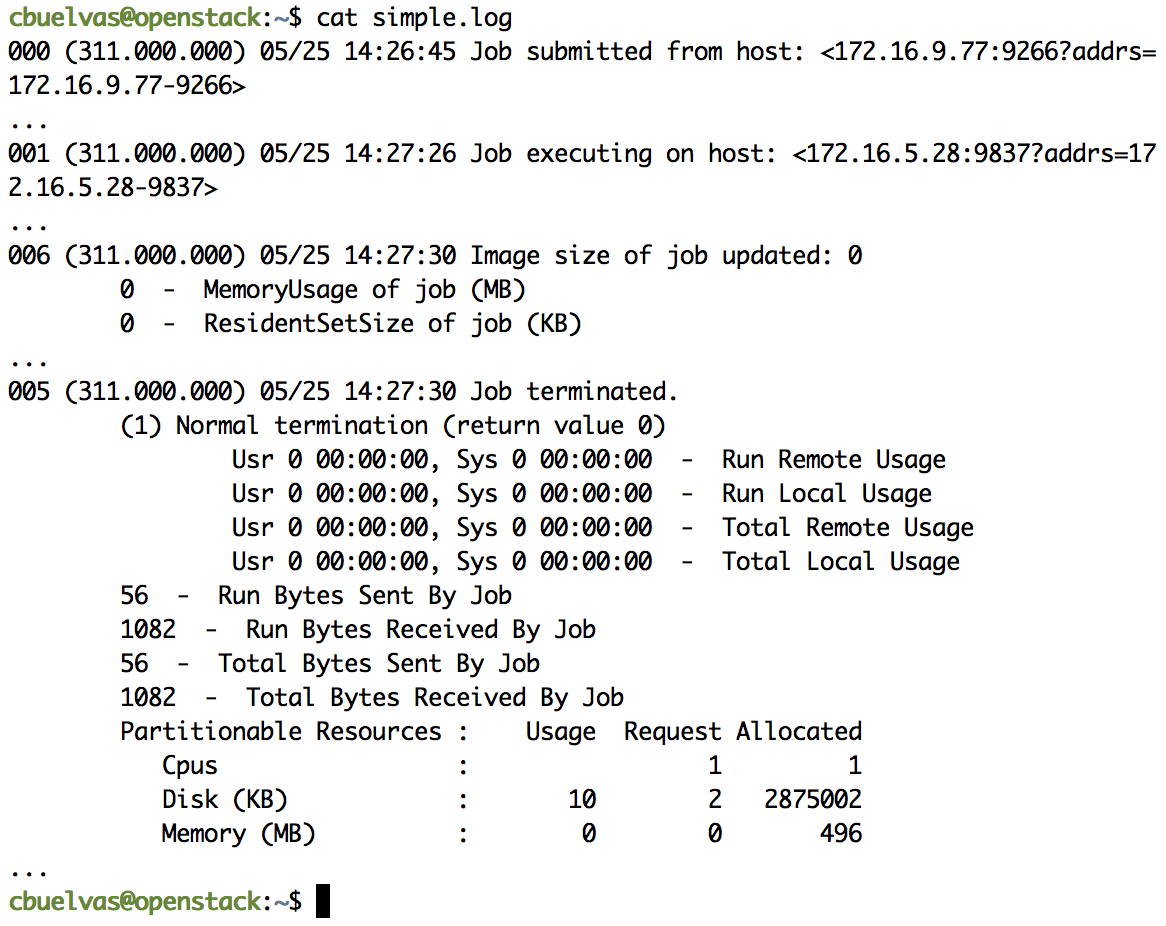
\includegraphics[width=0.9\textwidth]{images/sublog.png}
\decoRule
\caption{Log de envío}
\label{fig:file log}
\end{figure}
\FloatBarrier

Por ultimo verificamos el archivo de salida, que contiene los resultados de la ejecución.

\begin{figure}[h]
\centering
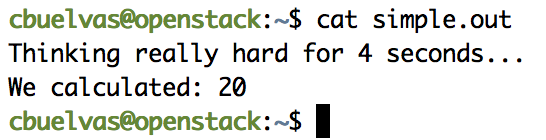
\includegraphics[width=0.8\textwidth]{images/simpleout.png}
\decoRule
\caption{Resultado prueba Java}
\label{fig:file log}
\end{figure}
\FloatBarrier

\section{Prueba de ejecución con Python}

Para esta prueba de ejecución, se calculara el tiempo de respuesta que le lleva a una maquina retornar el calculo y suma de los números primos en un rango dado. La prueba se ejecuta primero haciendo uso de multithreads y luego en serial, y arrojara el resultado en un archivos el cual se puede examinar una vez completado el trabajo.

\subsubsection*{Prueba en local}

El script que ejecutara el calculo es el siguiente:

\begin{lstlisting}[basicstyle=\footnotesize\ttfamily,
  language=Python, 
  numbers=left, 
  numberstyle=\tiny\color{black},
  captionpos=b]
#!/usr/bin/python
import multiprocessing as mp
from Queue import Empty
import math
import os
import time
def primeQ(n):
    """return a boolean, is the input integer a prime?"""
    if n == 2 :
        return True
    max =  int( math.ceil( math.sqrt(n) ) )
    i = 2
    while i <= max :
        if n % i == 0 :
            return False
        i += 1
    return True

def sumPrimes(n):
    """return sum of all primes less than n """
    return sum( [ x for x in range(2,n) if primeQ(x) ] )

def worker(q):
    while True:
        try:
            x = q.get(block=False)
            print sumPrimes(x)
        except Empty:
            break
if __name__ == "__main__":
    start = time.time()
ncpus = 4
my_q  = mp.Queue()
for i in range(100000, 2000000, 100000):
    my_q.put(i)
procs=[mp.Process(target=worker, args=(my_q,))  for i in range(ncpus)]
for ps in procs:
    ps.start()
for ps in procs:
    ps.join()
mid  = time.time()
print "now the serial part "
for i in range(100000, 2000000, 100000):
    print sumPrimes(i)
ending = time.time()
print "multiprocessing takes ", mid - start,      " seconds"
print "single thread takes ",      ending - mid,  " seconds"
\end{lstlisting}

Luego de creado el y editado el archivo se guarda el archivo como \textbf{primes} y se le da permisos de ejecución con el comando : \textbf{chmod a+x primes}.

Lo ejecutamos de manera local y vemos el resultado en la terminal:

\begin{figure}[h]
\centering
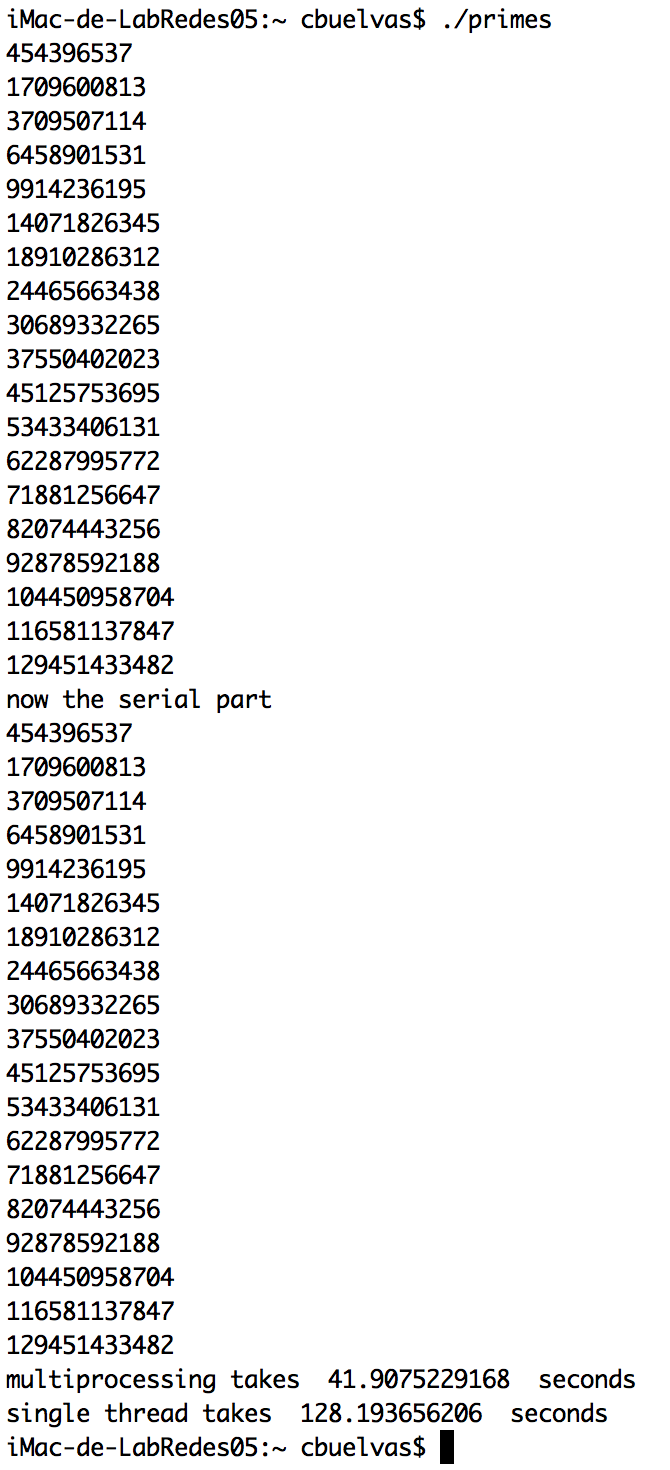
\includegraphics[width=0.8\textwidth]{images/localpython.png}
\decoRule
\caption{Ejecución de la prueba local}
\label{fig:python local test}
\end{figure}
\FloatBarrier

Luego llevamos este script a una máquina de envíos de trabajo y editamos el archivo ClassAd de envío y el script con la tarea.

Nuestro script es el mismo, se muestra como se configura el script para enviar las tarea:

\begin{figure}[h]
\centering
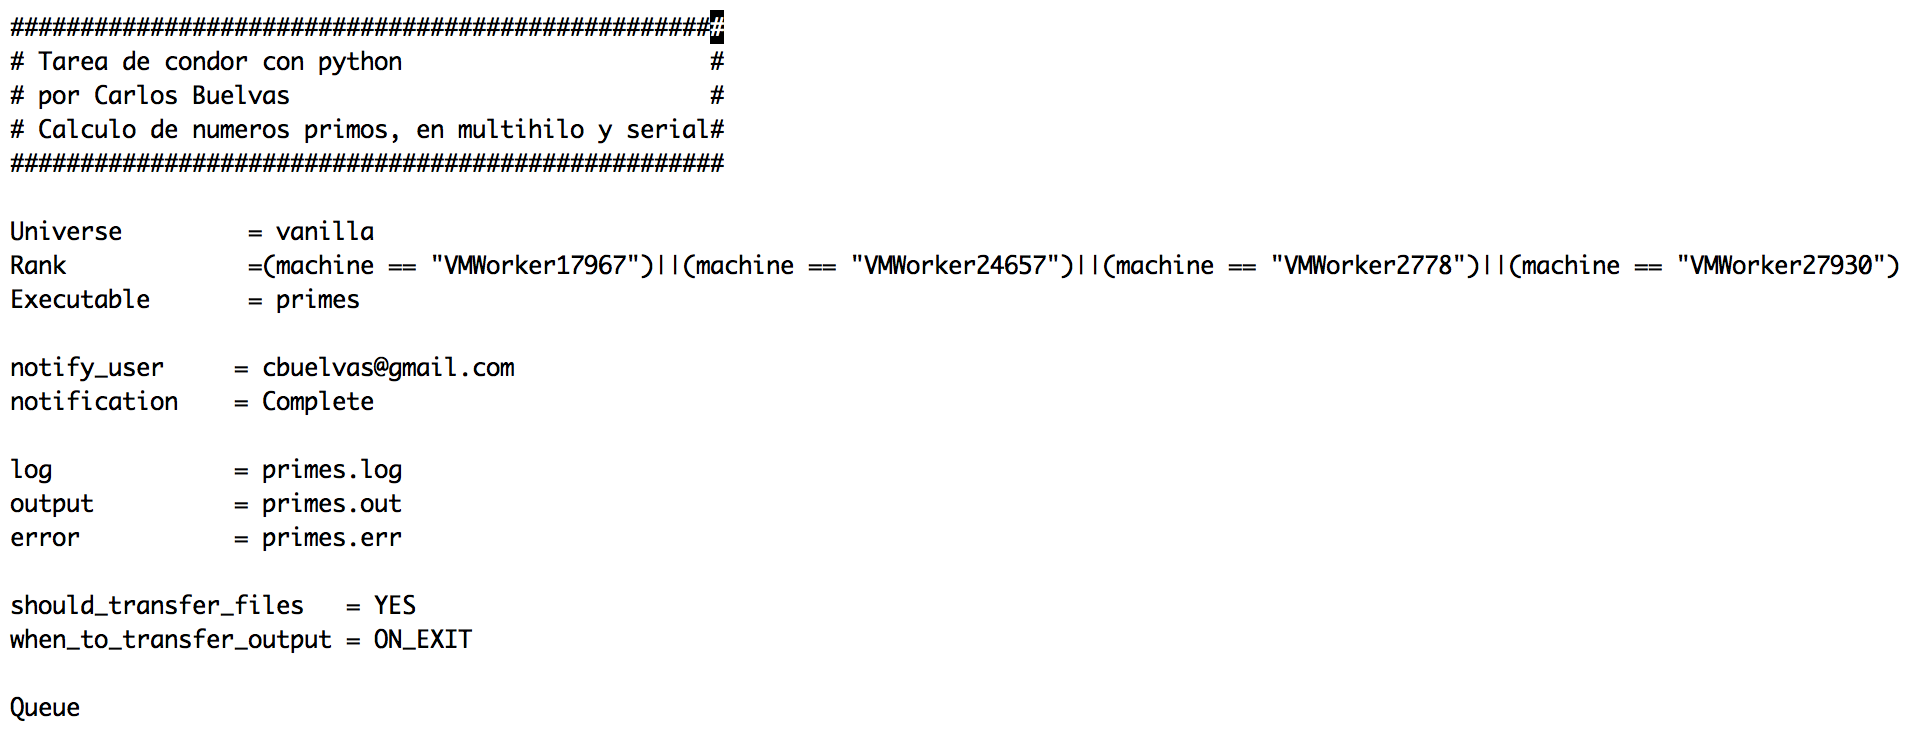
\includegraphics[width=1\textwidth]{images/pythonsub.png}
\decoRule
\caption{ClassAd para el envío al cluster}
\label{fig:python submit}
\end{figure}
\FloatBarrier

Enviamos el trabajo al cluster y verificamos que este en cola de trabajo.

\begin{figure}[h]
\centering
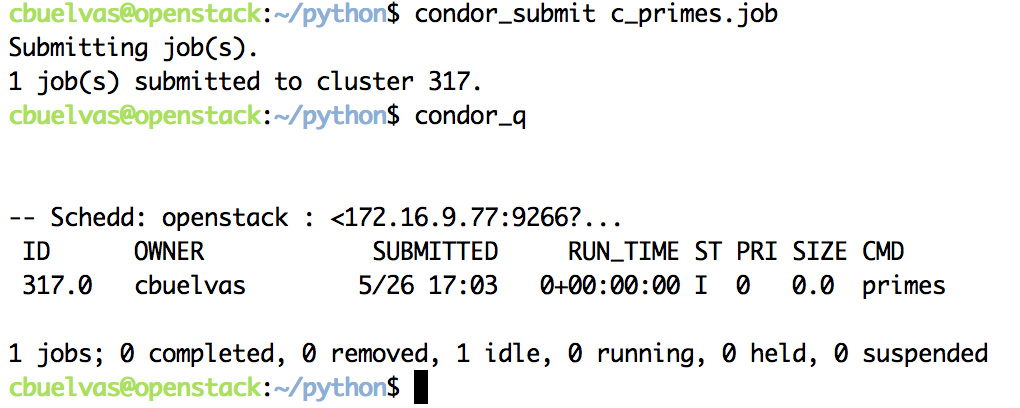
\includegraphics[width=0.8\textwidth]{images/condorsub.png}
\decoRule
\caption{Envío del trabajo y verificación de la cola de trabajos}
\label{fig:condor submit and q}
\end{figure}
\FloatBarrier

Luego podemos ver la información de la ejecución en el archivo de \textbf{\textit{log}}.
\begin{figure}[h]
\centering
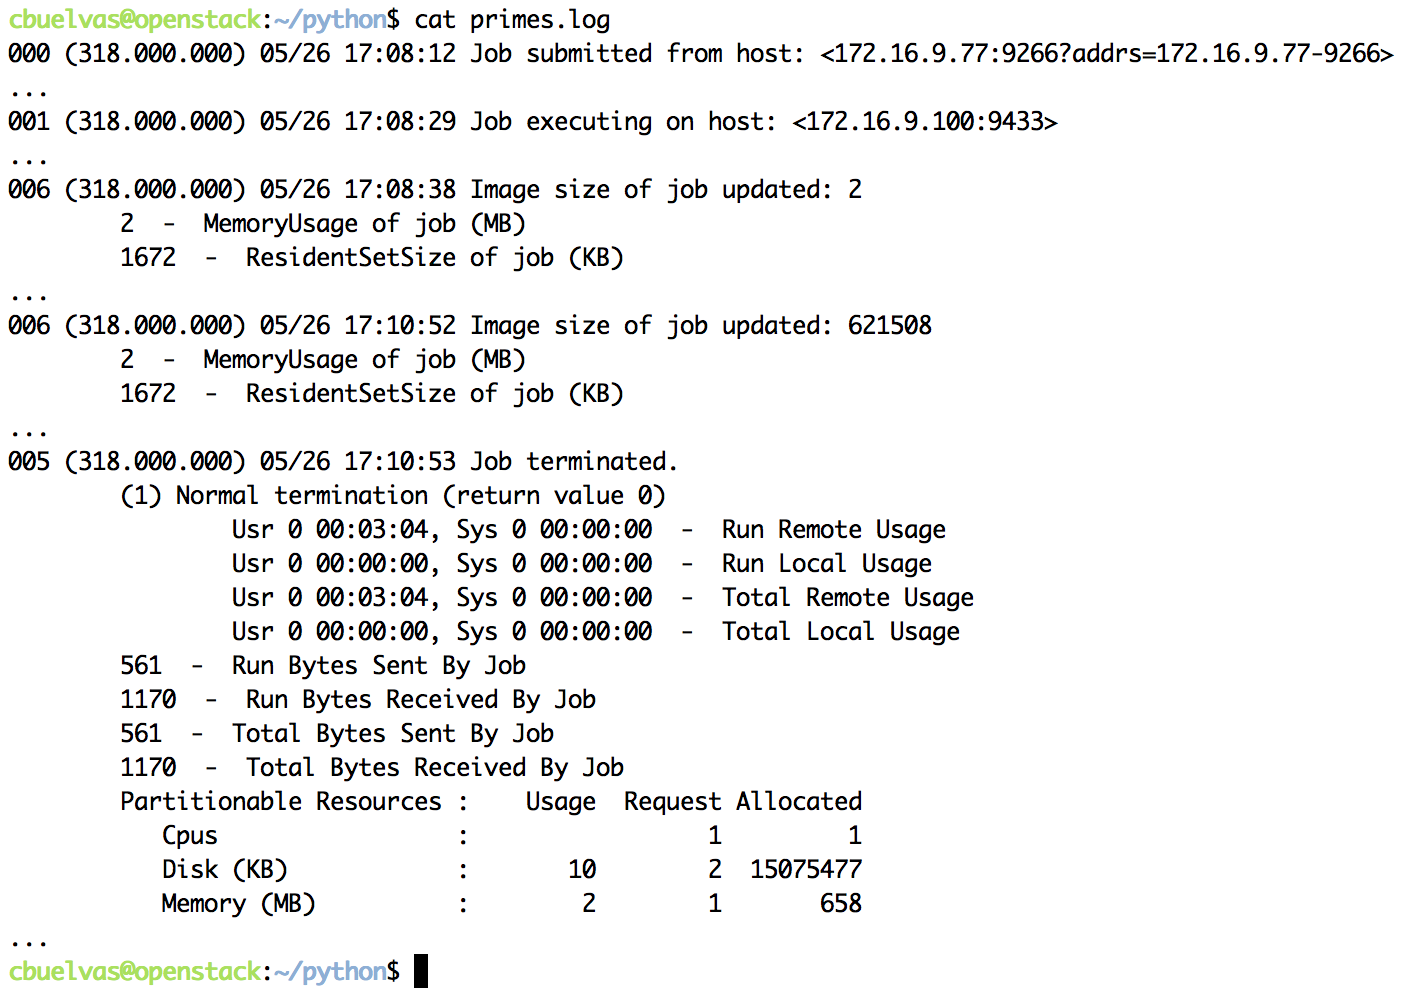
\includegraphics[width=1\textwidth]{images/pythonlog.png}
\decoRule
\caption{Log de ejecución de la prueba}
\label{fig:python log}
\end{figure}
\FloatBarrier
 Y el resultado de la ejecución lo vemos en el archivo de salida \textbf{\textit{.out}}.
 
 \begin{figure}[h]
\centering
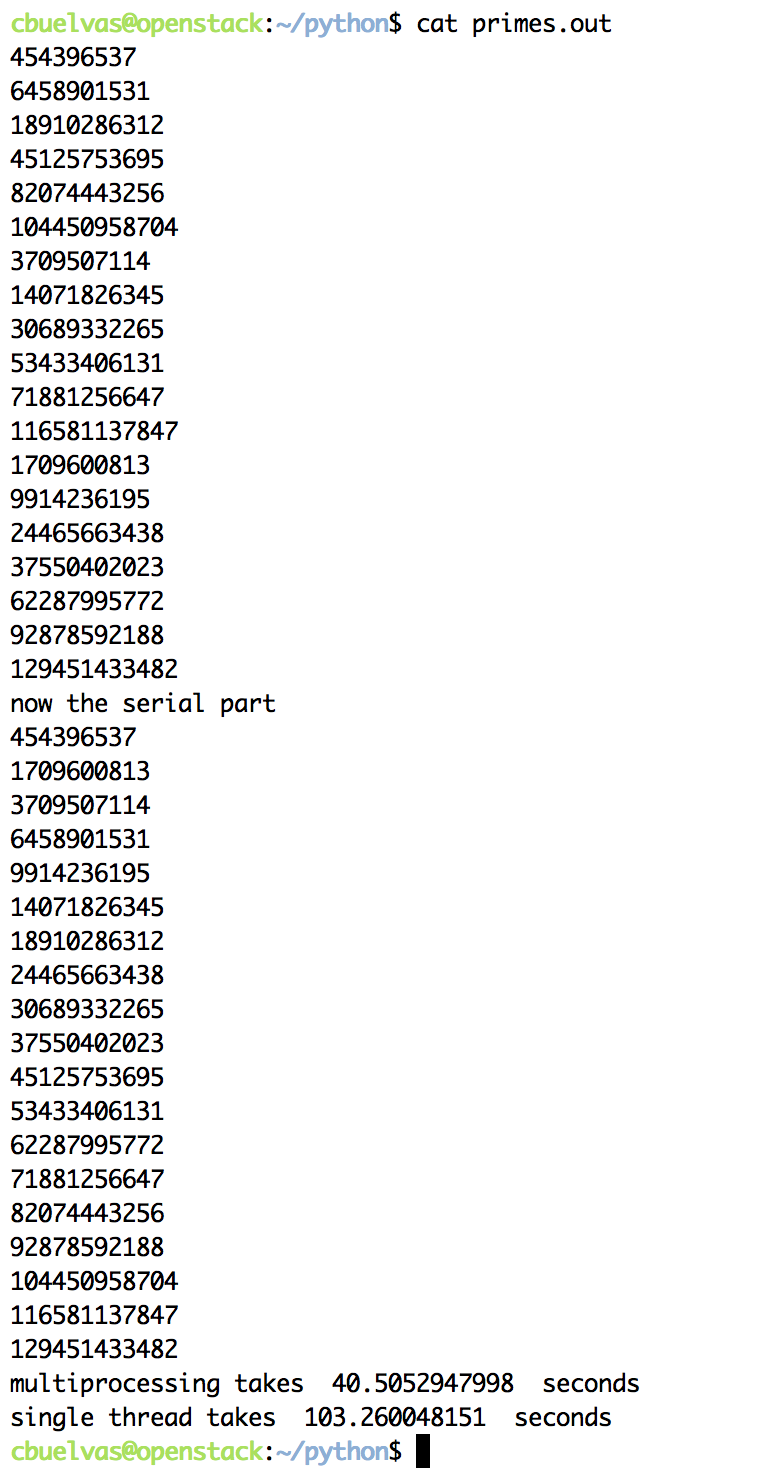
\includegraphics[width=0.8\textwidth]{images/clusterout.png}
\decoRule
\caption{Resultado de la ejecución}
\label{fig:python out}
\end{figure}
\FloatBarrier

con esto vemos que los entornos de ejecución para los cuales se diseño esta solución, están activos y son funcionales.

\section{Trabajos Futuros}

Al desarrollar este trabajo, se encontraron diferentes obstáculos a la hora de usar la herramienta HTCondor, entre ellas hay configuraciones de seguridad que se deben tener en cuenta.
\begin{itemize}
	\item Para lograr correcta comunicación entre los nodos de ejecución y el nodo maestro, todos deben pertenecer al mismo dominio (Ej, dominio.local.edu), para ello se deben configurar a la hora de instalar los equipos este dominio.
    \item Para aumentar la cantidad de nodos de trabajo, este trabajo se debe replicar en todos los salones de computo del campus.
    \item El nodo maestro, actualmente por pruebas esta aceptando los trabajos de cualquier dominio, esta es una falla de seguridad.
    \item Para hacer parte, y hacer uso de clusters de otras universidades, se debe configurar Flokking entre clusters.
\end{itemize}






%-----------------------------------------------